\chapter{Технологический раздел}
\label{cha:impl}

В данном разделе представлено проектирование анализатора поиска гонок и его реализация. Анализатор реализует метод статического поиска гонок на основе относительного множества блокировок.

\section{Выбор формы представления программы}

Большинство современных компиляторов, например, gcc, clang, поддерживают механизм трёхфазной компиляции, который состоит из:
\begin{itemize}
  \item преобразования исходного кода в промежуточное предствление,
  \item оптимизации промежуточного представления,
  \item получения кода целевой машины.
\end{itemize}
Каждому из этапов данного процесса компиляции соответствует своя форма представления программы: исходный код, промежуточное представление и код целевой машины. Отметим, что основным достоинством данного подхода является независимость процессов оптимизации и получения кода целевой машины от исходного языка программирования, на котором написана компилируемая программа. 

Исходный код программы является текстовым представлением программы на каком-либо высокоуровневом языке программирования. Разбор и анализ исходного кода программы является достаточно нетривиальной задачей в общем случае. Для этого обычно используются синтаксические анализаторы классов LL, LR или LALR. Кроме того, как правило, сложность построения графа потока управления в общем случае сводится к сложности синтаксиса языка в целом.

Промежуточное представление имеет достаточно простой ассемблероподобный синтаксис. Это сильно упрощает процессы разбора и анализа кода программы. В силу простоты синтаксиса языков промежуточного представления процесс построения графа потока управления становится весьма тривиальной задачей.

Код целевой машины является бинарным. В общем случае задача определения соответствия между кодом целевой машины и исходным кодом программы является нетривиальной, что может снизить информативность получаемых в процессе анализа результатов.

В силу описанных особенностей каждой из приведенных форм представления программы выбор был сделан в пользу использования промежуточного представления, т.к. информативность получаемых результатов и удобство проведения анализа являются наиболее важными свойствми при анализе. В качестве промежуточного представления был выбран Gimple IR, который используется наиболее распространённым в настоящее время компилятором gcc. 

\section{Выбор языка программивания. Используемые библиотеки}

В качестве языка программирования был выбран язык Python. Он хорошо подходит для создания прототипов работающих программ и обладает следующими достоинствами:
\begin{itemize}
  \item прост в изучении,
  \item позволяет решать сложные задачи,
  \item удобство сопровождения,
  \item высокая читаемость кода,
  \item высокая скорость разработки,
  \item превосходный синтаксис,
  \item поддержка объектно-ориентированного и структурного подходов программирования,
  \item поддержка функционального программирования,
  \item широкий спектр стандартных быблиотек,
  \item огромное количество сторонних свободно распространяемых библиотек с открытым исходным кодом,
  \item простой доступ к сторонним библиотекам, например, через PyPI (Python Package Index),
  \item кросплатформенность.
\end{itemize}

Основной используемой библиотекой является библиотека \textbf{gcc-python-plugin}. Она предоставляет возможность удобного написания загружаемых модулей для компилятора gcc на языке Python. Одним из немногих её недостатков является необходимость её сборки для конкретной платформы, на которой предполагается её использование.

\section{Написание плагинов для компилятора gcc}

Начиная с версии 4.5 компилятор gcc предоставляет API, предоставляющее возможность написания плагинов. Они являются загружаемыми модулями, позволяющими расширять базовую функциональность компилятора, например, выполнять преобразование кода, выполнять анализ и дополнительную оптимизацию кода и т.д.

Плагин запускается компилятором в момент возникновения определенных событий. Для каждого интересующего события в плагине необходимо выполнить регистрацию функции-обработчика обратного вызова (англ. callback function), которая будет вызвана компилятором при его возникновении. Перечень событий, для которых возможно выполнить регистрацию обработчика предстален в файле <<gcc\_plugin.h>>. Диаграмма последотельности, отражающая процесс взаимодействия между компилятором и плагином представлена на рис.~\ref{fig:sequence}.

\begin{figure}
  \centering
  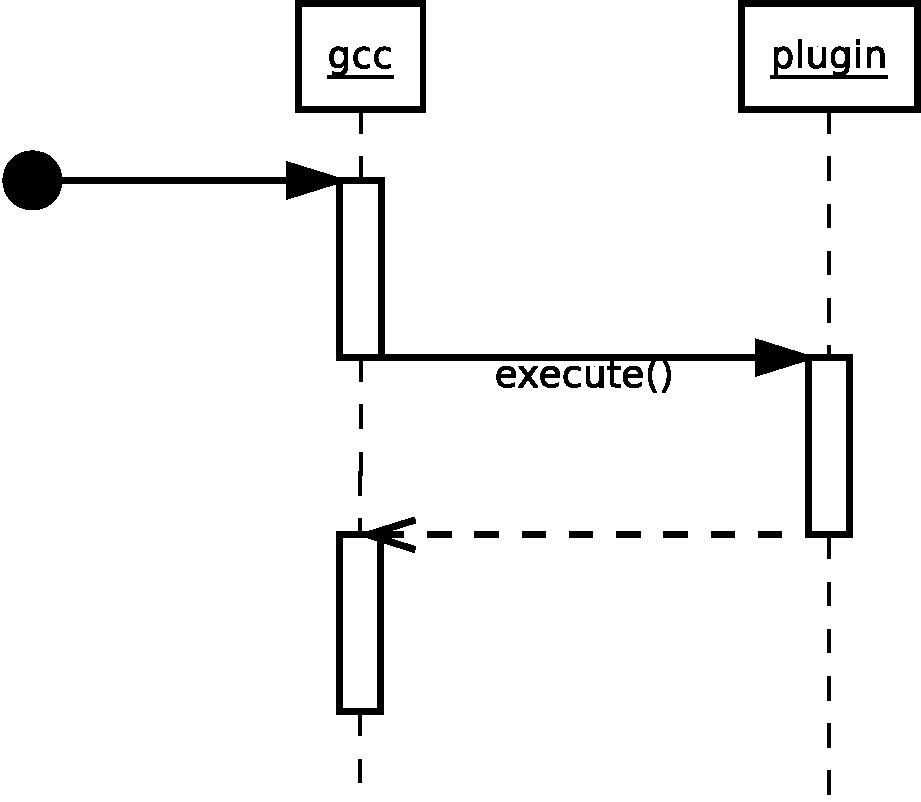
\includegraphics[width=0.5\textwidth]{inc/dia/sequence}
  \caption{Диаграмма последдовательности анализатора}
  \label{fig:sequence}
\end{figure}

\section{Ограничения реализации}

Для возможности реализации разработанного метода на анализируемый исходный код накладываются следующие ограничения:
\begin{itemize}
  \item использование POSIX API для работы с потоками и объектами взаимоисключения,
  \item отсутствие обращений к полям структур,
  \item уникальность имён переменных в пределах функции.
\end{itemize}

Создание потоков необходимо выполнять при помощи функции \textbf{pthread\_create}. Для взаимодействия с объектами синхронизации необходимо использовать следующие функции:
\begin{itemize}
  \item \textbf{sem\_wait} - ожидание освобождения и захват семафора,
  \item \textbf{sem\_post} - освобождение семафора,
  \item \textbf{pthread\_mutex\_lock} - захват мьютекса,
  \item \textbf{pthread\_mutex\_unlock} - освобождение мьютеса.
\end{itemize}


\section{Cтруктура ПО}

Разработанный статический анализатор кода выполнен в виде загружаемого модуля к компилятору gcc. Структура разработанного программного обеспечения представлена на рис.~\ref{fig:components}.

\begin{figure}
  \centering
  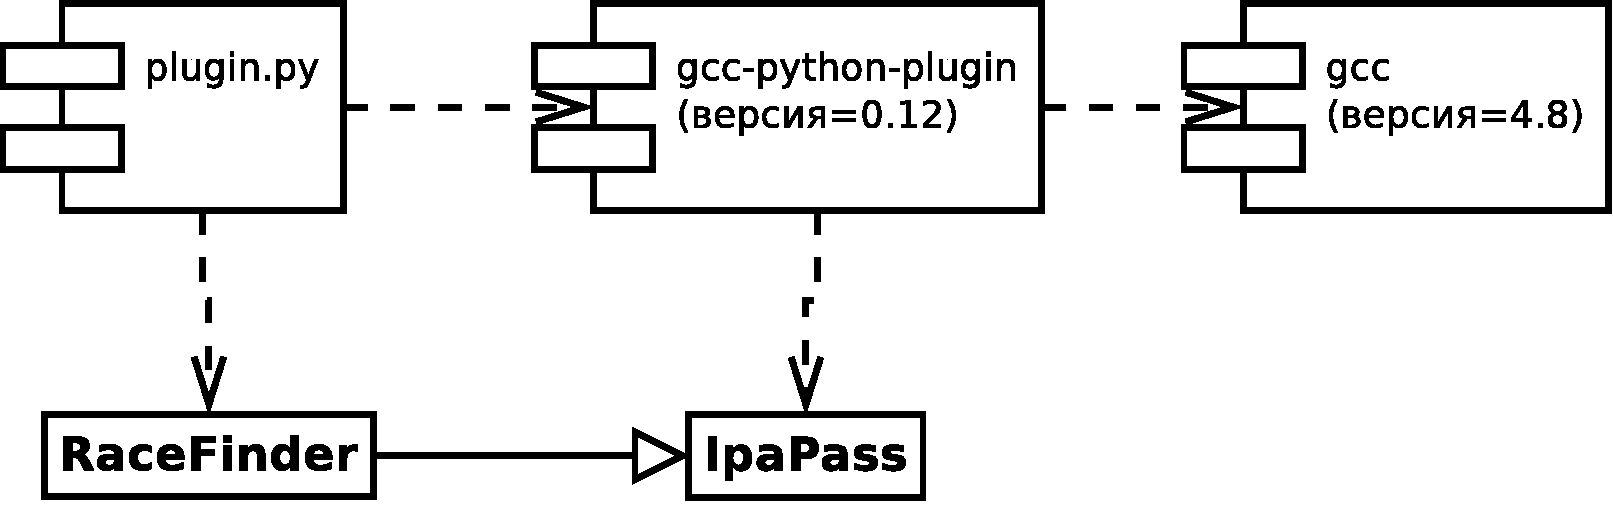
\includegraphics[width=\textwidth]{inc/dia/components}
  \caption{Диаграмма копонентов анализатора}
  \label{fig:components}
\end{figure}

\section{Запуск программы. Формат выходных сообщений}

Для запуска анализатора необходимо выполнить следующую команду к командной строке:
\begin{verbatim}
gcc -fplugin=<path-to-gcc-python-plugin-lib> \
    -fplugin-arg-python=plugin.py \
    -fplugin-arg-python-max-level=<max-level> \
    -fplugin-arg-python-with-main=<with-main> \
    <others>
\end{verbatim}
где:
\begin{itemize}
  \item <path-to-gcc-python-plugin-lib> - путь до библиотеки gcc-python-plugin,
  \item <max-level> - максимальное количество раз, которое базовый блок может встретиться в анализируемом пути,
  \item <with-main> - флаг, разрешающий/запрещающий включение в анализ результатов работы главного потока программа, допустимыми значениями которого являются строки $'true'$ и $'false'$,
  \item <others> - обычные параметры, задаваемые при компиляции программы c использованием компилятора gcc.
\end{itemize}

Пример запуска анализатора:
\begin{verbatim}
gcc -fplugin=/home/alex/gcc-python-plugin/python.so \
    -fplugin-arg-python=plugin.py \
    -fplugin-arg-python-max-level=1 \
    -fplugin-arg-python-with-main='true' \
    test.c -lpthread
\end{verbatim}

Сообщение о найденном месте возникновения гонки имеет следующий вид:
\begin{verbatim}
WARNING: Race condition when acccessing the variable <variable-name> (<visibility>) on line <line>
\end{verbatim}
где:
\begin{itemize}
  \item \textbf{<variable-name>} - имя переменной, к которой осуществлялся доступ,
  \item \textbf{<visibility} - область видимости переменной,
  \item \textbf{<line>} - строка, в которой производился доступ.
\end{itemize}

Пример сообщений, выдаваемых анализатором:
\begin{verbatim}
WARNING: Race condition when acccessing the variable buffer (global) on line 37
WARNING: Race condition when acccessing the variable buffer (global) on line 19
\end{verbatim}

\section{Выводы}

Разработано прораммное обеспечение, реализующее предложенный метод статического поиска гонок на основе относительного множества блокировок. Представлено обоснование выбора средств написания и библиотек для написания анализатора.
